\documentclass{report}

\usepackage{times}
\usepackage{helvet}
\usepackage{courier}
\usepackage{comment}
\usepackage{subfig}
\usepackage{relsize}
\usepackage[dvipdfmx]{graphicx}



\usepackage{enumitem}
\usepackage{adjustbox}
\usepackage{rotating}
\usepackage{multirow}
\usepackage{url}
\usepackage{listings}
\usepackage{lstlang0}

\usepackage{tikz} % Drawing sliding-tile

% Math
\usepackage{mathtools}
\usepackage{amsmath}
\usepackage{amsthm}
\usepackage{amssymb}
\usepackage[ruled,boxed,linesnumbered,noend]{algorithm2e}
\SetKwInOut{Input}{Input}
\SetKwInOut{Output}{Output}
\SetKwInOut{Side}{Side effect}
\SetKwComment{Comment}{$\triangleright$\ }{}

\newtheorem{definition}{Definition}
\newtheorem{theorem}{Theorem}

\setcounter{secnumdepth}{2}
%\frenchspacing

% Acronyms
\newcommand{\ZHDA}{ZHDA*}

% Utility macros: would be removed from the final version
\usepackage{newfloat}
\DeclareFloatingEnvironment{todo}

% Environments
\newenvironment{abst}[0]
	{
	\begin{quote}
	}
    {
	\end{quote}
	}

\title{ヒューリスティック探索}
\author{陣内 佑 \\
理化学研究所 革新知能統合研究センター}


\begin{document}

\maketitle
\listoftodos
\tableofcontents

\newpage

\section*{まえがき}
ヒューリスティック探索はグラフ探索のサブフィールドであり、解こうとしている問題の知識を探索方法に反映させることでより効率的に探索をしよう、という分野である。

ヒューリスティック探索のイントロダクションと現在どのように発展しているのかというのをまとめてみようかと思い、本文を執筆した。
以前、さる国内の高名なAI研究者がご講演で「ヒューリスティック探索は終わった技術であり、Toy Problemしか解けない」とおっしゃった。これは全くの勘違いであるが、思い返すと仕方がないことかと思われる。というのも、日本には探索分野、特にヒューリスティック探索の研究者というのは数えるほどしかいない。大御所の方々は大変忙しく、他分野、ましては自分では終わったと思っている分野の英語論文など読まないだろう。こうなると、その分野の知識は古いままで、なおのこと終わった分野だと思ってしまいがちである、と想像される。
そこで、若輩者ながら、数少ない日本語の書けるヒューリスティック探索アルゴリズムの研究者として、日本のAI研究に微力を添えようと日本語のテキストを書こうと思った次第である。


\chapter{イントロダクション}
\label{ch:introduction}

\captionlistentry[todo]{Introduction: なんかいい感じの絵}

人は様々な問題を探索によって解決している。
例えば飛行機で成田からロンドンに行く安い/速い方法などを計画するのは探索の一つである。
%一昔前は探索こそが人類の知であるという価値観が広くあり、囲碁、将棋、チェスなどのゲームはそれを競う競技であるとして。
あるいは囲碁、将棋、チェスなどのゲームも、ある手を選んだ時にどのような局面につながるのかを先読みし、選ぶべき次の一手を探索する。
このような様々な問題はグラフ探索問題として統合してモデルすることが出来る。
%もちろん、それぞれの問題はそれぞれの特徴があり、それぞれで効率的な解法が異なる。


% This chapter is ...
この章ではまず、\ref{sec:state-space-problem}節ではグラフ探索手法が用いられる問題として状態空間問題を定義する。
次に\ref{sec:search-problem}節で状態空間問題の例をいくつか紹介する。
経路探索問題や倉庫番問題など、応用がありつつ、かつ分かりやすい問題を選んだ。これらの問題はすべてヒューリスティック探索研究でベンチマークとして広く使われているものである。

\ref{sec:state-space-problem}節における定式化は\cite{russelln03}、\cite{pearl84}、\cite{edelkamp:2010:hst:1875144}などを参考にしている。本文は入門の内容であるので、研究の詳細が知りたい方はこれらの教科書を読むべきである。

\section{状態空間問題 (State-Space Problem)}
\label{sec:state-space-problem}
この本では主に初期状態とゴール条件が与えられたとき、ゴール条件を満たすための経路を返す問題を探索する手法を考える。
このテキストでは探索の主な対象として状態空間問題(State-space problem)を考える。状態空間問題$P = (S, A, s, T)$は状態の集合$S$、初期状態$s \in S$、ゴール集合$T \in S$、アクション集合$A = {a_1, ....,a_n}$、$a_i : S \rightarrow S$がある。アクションはある状態を次の状態に遷移させる関数である。
状態空間問題の解は初期状態からゴール状態へ遷移させるアクションの列を求めることである。

よって、状態空間問題はグラフにモデルすることで考えやすくなる。
状態空間グラフは以下のように定義される。

\begin{definition}[状態空間グラフ、State-space graph]
問題グラフ$G = (V, E, s, T)$は状態空間問題$P = (S, A, s, T)$に対して以下のように定義される。ノード集合 $V = S$、初期ノード$s \in S$、ゴールノード集合$T$、エッジ集合$E\subseteq V \times V$。エッジ$u,v\in E$は$a(u) = v$となる$a\in A$が存在する場合に存在し、そしてその場合にのみ存在する(iff)。
\end{definition}

状態空間問題の解は以下の定義である。

\begin{definition}[解、Solution]
解$\pi = (a_1,a_2...,a_k)$はアクション$a_i \in A$の(順序付)配列であり、初期状態$s$からゴール状態$t \in T$へ遷移させる。すなわち、$u_i \in S$,$i \in \{0,1,...,k\}$, $u_0 = s, u_k = t$が存在し、$u_i = a_i(u_{i-1})$となる。
\end{definition}

どのような解を見つけたいかは問題に依存する。
多くの問題では経路の{\bf コスト}の合計を小さくすることを目的とする。

%すなわち、アクションに対してコストが定義されており、経路

\begin{definition}[コスト付き状態空間問題、Weighted state-space problem]
コスト付き状態空間問題$P = (S, A, s, T, w)$は状態空間問題の定義に加え、コスト関数$w: A \rightarrow \mathbb{R}$がある。経路$(a_1,...,a_k)$のコストは$\sum^k_{i=1}w(a_i)$と定義される。ある解が可能なすべての解の中でコストが最小である場合、その解を最適解(optimal cost solution)であると言う。
\end{definition}

本書ではコスト付き状態空間問題をメインの問題として考える。
%最適解が欲しいかどうかは問題による。当然クオリティが高い解を得ようとするとより計算に時間とメモリを消費することになる。

コストの定義されていない状態空間問題を特に区別してユニットコスト問題(ユニットコストドメイン)と呼ぶ。
コスト付き状態空間問題は重み付き(コスト付き)グラフとしてモデルすることが出来る。すなわち、$G = (V, E, s, T, w)$は状態空間グラフの定義に加え、エッジの重み$w: E \leftarrow \mathbb{R}$を持つ。



%ただし、状態空間グラフをすべて陽に変換し、すべてのノード・エッジを保持することは効率が良くないことが多い。
\ref{ch:blind-search}章で詳解するが、探索アルゴリズムは状態空間グラフのノード・エッジ全てを保持する必要はない。
全てのノード・エッジを保持した状態空間グラフを特に明示的状態空間グラフ(explicit state-space graph)と呼ぶとする。このようなグラフは、例えば隣接行列を用いて表すことが出来る。隣接行列$M$は行と列の大きさが$|V|$である正方行列であり、エッジ$(v_i, v_j)$が存在するならば$M_{i,j}=1$、なければ$M_{i,j}=0$とする行列である。
このような表現方法の問題点は行列の大きさが$|V|^2$であるため、大きな状態空間を保持することが出来ないことである。
例えば、\index{sec:search-problem}節で紹介する15-puzzleは状態の数が$|V|=15!/2$であるため、隣接行列を保持することは現在のコンピュータでは非常に困難である。

そこで、探索アルゴリズムは多くの場合初期ノードとノード展開関数による非明示的状態空間グラフで表せられる。

\begin{definition}[非明示的状態空間グラフ、Implicit state-space graph]
非明示的状態空間グラフは初期状態$s \in V$、ゴール条件Goal: $V \rightarrow B = \{false, true\}$、ノード展開関数Expand: $V \rightarrow 2^V$によって与えられる。
\end{definition}

探索の開始時、エージェントは初期ノードのみを保持する。エージェントは保持しているノードに対してExpandを適用することによって、新しいノードとエッジをグラフに加える。これを求める解を見つけるまで繰り返す。
Expandはある状態からの次の状態の集合を返す関数である。Expand関数は明示的に与えられるのではなく、ルールによって与えられることが多い。例えば将棋であれば、将棋のルールによって定められる合法手によって得られる次の状態の集合がExpand関数によって得られる。
これによって、エージェントは解を見つけるまでのノード・エッジだけ保持して必要な解を見つけることが出来る。


%\begin{example}

%\end{example}

%大まかには、情報なし探索による非明示的グラフは明示的グラフよりも指数的に小さく、ヒューリスティック探索による非明示的グラフは情報なし探索による非明示的グラフよりも更に指数的に小さいことが多い。



% TODO: アルゴリズムを表にする?

\section{状態空間問題の例}
\label{sec:search-problem}

状態空間問題の例をいくつか紹介する。
グリッド経路探索問題や倉庫番問題など、応用がありつつ、かつ分かりやすい問題を選んだ。これらの問題はすべてヒューリスティック探索研究でベンチマークとして広く使われているものである。
%グラフ探索アルゴリズムによって効率的に解くことが出来ると知られているドメインをいくつか紹介する。
%ここで詳解する問題はグラフ探索以外の手法でも解くことが出来る。


\subsection{グリッド経路探索 (Grid Path-finding)}
\captionlistentry[todo]{Grid Pathfinding: なんかいい感じの絵}
グリッド経路探索問題は$k$(多くの場合$k=2$)次元のグリッド上で初期配置からゴール位置までの経路を求める問題である。グリッドには障害物がおかれ、通れない箇所がある。エージェントが移動できる方向は4方向($A= \{up, down, left, right\}$)か8方向(4方向に加えて斜め移動)とする場合が多い。

Web上に簡単に試せるデモがあるので、参照されたい:\url{http://qiao.github.io/PathFinding.js/visual/}。とてもよくできており、この文章で説明する様々なグラフ探索手法をグリッド経路探索に試すことが出来る。

グリッド経路探索はゲームAIなどで応用される。ストラテジーゲームなどでユニット(エージェント)を動かすために使われる。
またグリッドは様々な問題を経路探索に帰着して解くことができるという意味でも重要である。例えばMultiple Sequence Alignmentはグリッド経路探索に帰着して解くことが出来る(後述)。
あるいはロボットのモーションプランニングなども経路探索となる。すなわち、$k$個の関節の角度を変えて、現在状態からゴール状態へ遷移させたい。各関節の角度がグリッドの各次元に相当する。ロボットの物理的な構造により、関節のある角度の組み合わせは不可能である。不可能な組み合わせが、障害物の置かれたグリッドに相当する。よって、障害物を避けた経路というのが関節の動かし方ということになる。

%Starcraft 1ではA*探索が使われていた。
%しかしマルチエージェント
%マルチエージェント経路探索の場合はflocking / swarm AIが使われている。Starcraft 2では


\subsection{スライディングタイル (Sliding-tile Puzzle)}

多くの一人ゲームはグラフ探索問題に帰着することが出来る。スライディングタイルはその例であり、ヒューリスティック探索研究においてメジャーなベンチマーク問題でもある (図\ref{fig:15-puzzle})。
$1$から$(n^2)-1$までの数字が振られたタイルが$n\times n$の正方形に並べられている。正方形には一つだけ{\it ブランク}と呼ばれるタイルのない位置があり、四方に隣り合うタイルのいずれかをその位置に移動する(スライドする)ことが出来る。スライディングタイル問題は、与えられた初期状態からスライドを繰り返し、ゴール状態にたどり着く経路を求める問題である。

\begin{figure}
\centering
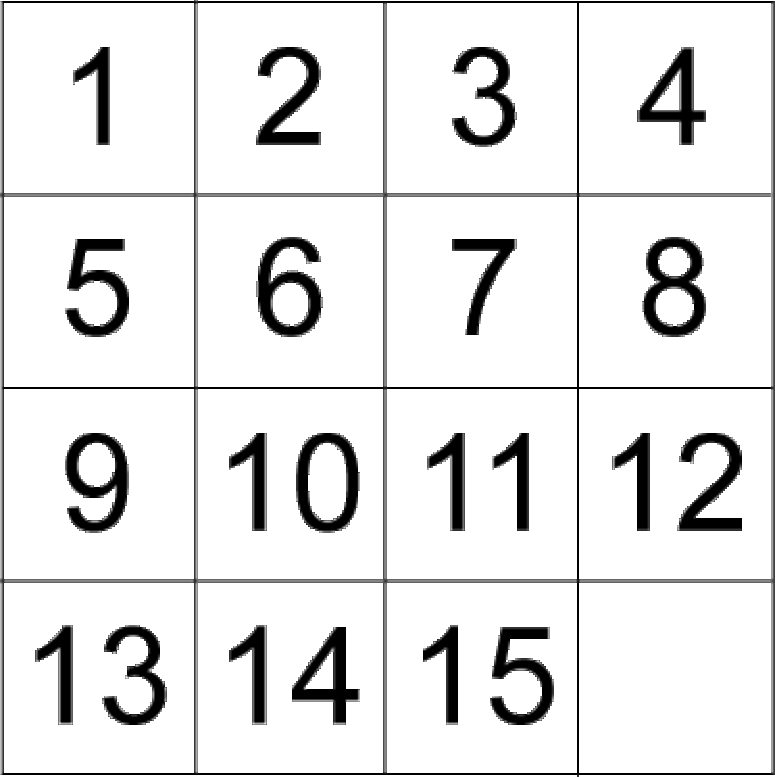
\includegraphics[width=0.4\textwidth]{figures/15-puzzle.pdf}
\caption{15パズルのゴール状態の例}
\label{fig:15-puzzle}
\end{figure}

スライディングタイルの到達可能な状態の数は$|V| = (n^2)!/2$\footnote{スライディングタイルは偶奇性があり、到達不可能な状態がある\cite{TODO}。}であり、$n$に対して指数的に増加する。
可能なアクションは$A= \{up, down, left, right\}$の4つであり、アクションにかかるコストはすべて同じとする。

後述するが、ヒューリスティック探索のためには状態からゴール状態までの距離(コスト)の下界(lower bound)を計算する必要がある。
スライディングタイルにおける下界の求め方として最もシンプルなものは{\it マンハッタン距離ヒューリスティック}である。マンハッタン距離ヒューリスティックは各タイルの現在状態の位置とゴール状態の位置のマンハッタン距離の総和を取る。可能なアクションはすべて一つしかタイルを動かさないので、一回のアクションでマンハッタン距離は最大で1しか縮まらない。よって、マンハッタン距離はゴールまでの距離の下界である。

%ちなみに、スライディングタイルはpermutation problemの一つである。

\subsection{Multiple Sequence Alignment (MSA)}

生物学・進化学では遺伝子配列・アミノ酸配列の編集距離(edit distance)を比較することでニ個体がどれだけ親しいかを推定することが広く研究されている。
MSAは複数の遺伝子・アミノ酸配列が与えられた時、それらの配列間の編集距離とその時出来上がった配列を求める問題である。
2つの配列に対してそれぞれコストの定義された編集操作を繰り返し、同一の配列に並べ替える手続きをアライメントと呼ぶ。
2つの配列の編集距離はアライメントのコストの最小値である。
3つ以上の配列における距離の定義は様々考えられるが、ここでは全ての配列のペアの編集距離の総和を用いる。

MSAにおける可能な編集操作は置換と挿入である。置換は配列のある要素(DNAかアミノ酸)を別の要素に入れ替える操作であり、挿入は配列のある位置に要素を挿入する操作である。例えば(ABC, BCB, CB)の3つの配列のアライメントを考える。図\ref{fig:msa-cost}は置換と編集に対するコストの例である。-は欠損、すなわち挿入操作が行われたことを示す。アミノ酸配列における有名なコスト表としてPAM250があるが、ここでは簡単のため仮のコスト表を用いる\cite{MSA}。
図\ref{fig:msa-solution}はこのコスト表を用いたアライメントの例である。
このとき、例えば配列ABC-と-BCBの編集距離は(A,-)、 (B,B)、 (C,C)、 (-,B)のコストの総和であるので、図\ref{fig:msa-cost}を参照し、$5+0+1+5=11$である。(-BCB, --CB)の距離は$6$, (--CB, ABC-)の距離は$16$であるので、3配列の編集距離は$11+6+16=33$である。

$n$配列のMSAは$n$次元のグリッドの経路探索問題に帰着することが出来る。
図\ref{fig:msa-to-grid}は(ABC)と(BCB)の2つの配列による問題を表す。
状態$s$は2つの変数によって表現される:$(x_0, x_1)$。$x_0$は配列0のどの位置までアライメントを完了したかを表す変数であり、配列$i$の長さを$l_i$とすると定義域は$0 \leq x_0 \leq l_0$である。
全てのアライメントが完了した状態$s=(l_0, l_1)$がゴール状態である。
可能なアクションは$a=(b_0, b_1), (b_i=0, 1)$の形を取り、これは配列$i$に対して欠損を挿入する場合に$b_i=0$となる。
状態$s$に対してアクション$a$を適用した後の状態$s'$は$s'=(x_0+b_0, x_1+b_1)$となる。例えば図\ref{fig:msa-to-grid}は初期状態$s=(0,0)$に対して$a=(1,0)$を適用している。これは(A), (-)までアライメントを進めた状態に対応する。次に$a=(1,1)$が適用され、アライメントは(A,B), (-,B)という状態に至る。

このようにして、MSAはグリッド経路探索問題に帰着し、グラフ探索アルゴリズムよって解くことが出来る。
状態空間問題として考えた場合にMSAの難しさはアクションのコストが幅広いことにある。また、分枝数は配列の数$n$に対して$2^n-1$と大きい。

MSAは生物学研究に役立つというモチベーションから非常に熱心に研究されており、様々な定式化による解法が知られている。
例えば動的計画法が使われている。



\begin{figure}
\centering
\subfloat[MSAの解の例]{
\begin{tabular}{ccccc}
	A & B & C & - \\
	- & B & C & B \\
	- & - & C & B \\
\end{tabular}
\label{fig:msa-solution}
} \hspace{4pt}
\subfloat[操作コスト表の例]{
\begin{tabular}{c|cccc}
	  & A & B & C & - \\ \hline
	A & 0 & 1 & 2 & 5 \\
	B &   & 0 & 3 & 5 \\
	C &   &   & 1 & 5 \\
	- &   &   &   & 0 \\	
\end{tabular}
\label{fig:msa-cost}
} \hspace{4pt}
\subfloat[グリッド経路探索への帰着]{
\begin{tabular}{c|cccc}
	  &   & A & B & C \\ \hline
	  & $\rightarrow$ & $\searrow$ &   &   \\
	B &   &   & $\searrow$ &   \\
	C &   &   &   & $\downarrow$ \\
	B &   &   &   & $\searrow$ \\
\end{tabular}
\label{fig:msa-to-grid}
}
\subfloat[グリッド経路探索への帰着]{
\begin{tabular}{c|cccc}
	  & A & B & C & - \\ \hline
	  & - & B & C & B \\ \hline
\end{tabular}
\label{fig:msa-to-grid-align}
}
\end{figure}



\subsection{倉庫番 (Sokoban)}
倉庫番(Sokoban)は日本発のパズルゲームであり、倉庫の荷物を押していくことで指定された位置に置くというゲームである。現在でも様々なゲームでゲーム内ミニゲームとして親しまれている。
プレイヤーは「荷物の後ろに回って押す」ことしか出来ず、引っ張ったり、横から動かしたりすることが出来ない。また、荷物の上を通ることも出来ない。

\begin{figure}
\centering
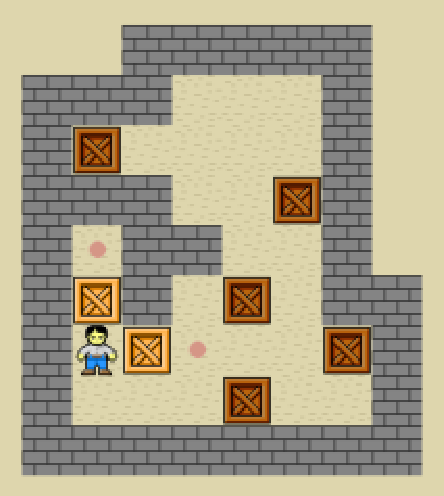
\includegraphics[width=0.4\textwidth]{figures/sokoban.pdf}
\caption{Sokoban: 画像はwikipediaより。}
\label{fig:sokoban}
\end{figure}

状態の表現方法は2通りあり、一つはグリッドの各位置に何が置いてあるかを変数とする方法である。もうひとつはプレイヤー、各荷物の位置に対してそれぞれ変数を割り当てる方法である。
可能なアクションは$\{move-up,move-left,move-down,move-right,push-up,push-left,push-down,push-right\}$の8通りである。$move-*$はプレイヤーが動くアクションに対応し、コストは0である。$push-*$は荷物を押すアクションであり、正のアクションコストが割当てられている。よって、倉庫番はなるべく荷物を押す回数を少なくして荷物を目的の位置に動かすことが目的となる。

グラフ探索問題として倉庫番を考えるときに重要であるのは、倉庫番は{\it 不可逆な}アクション(irreversible)があることである。
グリッド経路探索やスライディングタイルは{\it 可逆な} (reversible)問題である。
全てのアクション$a \in A$に対して$a^{-1} \in A$が存在し、$a(a^{-1}(s)) = s$かつ$a^{-1}(a(s)) = s$となる場合、問題は可逆であると言う。
可逆な問題は対応するアクションのコストが同じであれば無向グラフとしてモデルすることも出来、初期状態から到達できる状態は、すべて初期状態に戻ることが出来る。
一方、不可逆な問題ではこれが保証されず、詰み(trap)状態に陥る可能性がある。

倉庫番では荷物を押すことは出来ても引っ張ることが出来ないため、不可逆な問題である。例えば、荷物を部屋の隅に置いてしまうと戻すことが出来ないため、詰み状態に陥る可能性がある問題である。
このような性質を持つ問題では特にグラフ探索による先読みが効果的である。

もうひとつ重要な問題はゼロコストアクションの存在である。%TODO
倉庫番のアクションのうち$\{move-up,move-left,move-down,move-right\}$はコストゼロ($w(e)=0$)のアクションである。ヘタなアルゴリズムを実行すると無限に無駄なアクションを繰り返し続けるということもありうるだろう。


%倉庫の中には荷物がおかれ、エージェント(プレイヤー)は迷路を動き回り、
%このゲームで面白い/難しいのは、「荷物の後ろに回って押す」ことしか出来ず、引っ張ったり、横から動かしたりすることが出来ないという点である。

\subsection{巡回セールスパーソン問題 (Traveling Salesperson Problem, TSP)}

セールスパーソンはいくつかの都市に回って営業を行わなければならない。都市間の距離(=コスト)は事前に与えられている。
TSPは全ての都市を最短距離で回ってはじめの都市に戻る経路を求める、という問題である。

\begin{figure}
\centering
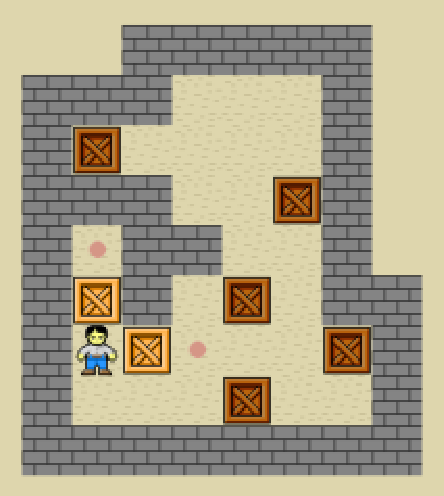
\includegraphics[width=0.4\textwidth]{figures/sokoban.pdf}%TODO
\caption{巡回セールスパーソン問題: 画像はwikipediaより。}
\label{fig:sokoban}
\end{figure}
\captionlistentry[todo]{巡回セールスマン問題: 画像を挿入}

$n$個の都市があるとすると(最適・非最適含む)解の数は$(n-1)!/2$個である。
可能なアクションは「都市$i \in \{1..n\}$を訪れる」であり、一度訪れた都市には行けない。
TSPのゴール条件はすべての都市を訪れることである。よって、$n$回どれかアクションを実行すれば、とりあえず解を得ることが出来る。一方、最適解を得る問題はNP完全であることが知られている。

TSPの解の下界としては{\it 最小全域木} (minimum spanning tree)のコストがよく用いられる。
グラフの{\it 全域木} (spanning tree)は全てのノードを含むループを含まない部分グラフである。
最小全域木は全域木のうち最もエッジコストの総和が小さいものである。
未訪問の都市によるグラフの最小全域木はTSPの下界となることが知られている。

TSPはヒューリスティック探索に限らず、様々なアプローチで研究されている問題ドメインである\cite{applegate2006traveling}。この問題ドメインについて特に詳しく知りたい方はそちらの教科書を参照されたい。


%%%%%%%%%%%%%%%%%%%%%%%%%%%%%%%%%%%%%%%%%%%%%%%%%
%%% CHAPTER: Blind Search
%%%%%%%%%%%%%%%%%%%%%%%%%%%%%%%%%%%%%%%%%%%%%%%%%
\chapter{情報なし探索 (Blind Search)}
\label{ch:blind-search}

\ref{ch:introduction}章では様々な状態空間問題を紹介したが、それぞれの問題の解法はどれも沢山研究されている。
一つの指針としては、ある問題に特化した解法を研究することでその問題をより高速に解くというモチベーションがある。
これは例えばMSAのように重要なアプリケーションがある問題の場合に特に熱心に研究されることが多い。
一方、なるべく広い範囲の問題に対して適用可能な手法を研究するというモチベーションもある。
特に人工知能の文脈において、なるべく問題の知識を必要とせず、最小限の仮定のみを必要とする解法が求められる。
%ただしこのような手法はドメインに特化したプログラムと比べてパフォーマンスに劣ることが多い。

\ref{ch:introduction}章で紹介した状態空間問題を広く扱うことの出来る手法としてグラフ探索アルゴリズムがある。
本章では最もシンプルな問題(ドメイン)の知識を利用しない探索を紹介する。
情報なし探索 (Blind Search)は状態空間グラフのみに注目し、背景にある問題に関する知識を一切使わないアルゴリズムである。
情報なし探索で重要なのは1. 重複検知を行うかと 2. ノードの展開順序の二点である。
重複検知は訪問済みのノードを保存しておくことで同じノードを繰り返し探索することを防ぐ手法である。対価としては、メモリの消費量が非常に大きくなることにある。
ノードの展開順序とは、例えば幅優先探索・深さ優先探索などのバリエーションを指す。
効率的な展開順序は問題によって大きく異なり、問題を選べばこれらの手法によって十分に効率的な探索を行うことが出来る。
これらの探索手法は競技プログラミングでもよく解法として使われる(らしい)\footnote{TODO: 典拠}。また、いわゆるコーディング面接でもグラフ探索アルゴリズムは頻出である(らしい)\footnote{TODO: 典拠}。
%\ref{ch:search-performance}章はグラフ探索の高速化の紹介をするので、特に競技プログラミングに興味がある場合はそちらも参照されたい。% TODO



\section{木探索アルゴリズム (Tree Search Algorithm)}
\label{sec:tree-search-algorithm}
木探索アルゴリズムはグラフ探索アルゴリズムの基礎となるフレームワークであり、本文で紹介する手法のほとんどがこのフレームワークを基礎としているといえる。

アルゴリズム\ref{alg:implicit-tree-search}は木探索の疑似コードである。

\begin{algorithm}
\caption{Implicit Tree Search}
\label{alg:implicit-tree-search}
	\Input{initial node $s$, weight function $w$, successor generation function $Expand$, goal function $Goal$}
	\Output{Path from $s$ to a goal node $t \in T$, or $\emptyset$ if no such path exists}
	$Open \leftarrow \{s\}$\;
	\While{$Open \neq \emptyset$} {
		$u \leftarrow Open.pop()$\;
		\If {$Goal(u)$} {
			\Return $Path(u)$\;
		}
		$Succ(u) \leftarrow Expand(u)$\;
		\For {each $v \in Succ(u)$} {
			$Open.insert(v)$\;
			$parent(v) \leftarrow u$\;
		}
 	}
	\Return $\emptyset$\;
\end{algorithm}

以下、(k)と書いて疑似コードのk行目を指すことにする。
木探索はオープンリスト\footnote{歴史的な経緯でリストと呼ばれているが、データ構造がリストで実装されるという意味ではない。}と呼ばれるノードの集合を保持する。探索の開始時には、初期状態のみがオープンリストに入っている(1)。
木探索は、このオープンリストから一つノード$u$を選び(3)、ゴール条件を満たしているかを確認する(4)。満たしていれば初期状態から$u$への経路を返す。満たしていなければ、そのノードを展開する(6-)。展開とは、そのノードの子ノードを列挙し、オープンリストに入れる(8)ことを指す。

探索の進行によってエージェントが保持する情報は変化していく。ここでは探索がどのように進行するかを記述するため、以下の3つの言葉を定義する:

\begin{enumerate}
\item 展開済みノード: $Expand(u)$によって子ノードが参照されたノードを指す。$Open$からは省かれる。
\item 生成済みノード: $Open.insert(v)$によってOpenに一度でも入れられたノードを指す。
\item 未生成ノード: まだ生成されていないノード。よって、非明示的グラフに保持されていない。

\end{enumerate}

非明示的グラフ木探索の強みは、生成済みノードのうち展開済みではないもののみを$Open$に保持すればよいことにある。未生成ノード、展開済みノードはメモリ上に保持する必要がない。
$Open$はPriority queueであり、何らかの基準によって$Open$から取り出してくるノードを決める。

木探索アルゴリズムは名前の通り木を探索する場合により効率的であることが多いが(後述するが、重複検出をしないため)、グラフ一般に対して適用することが出来る。


%同じ状態を複数回展開すると計算資源を無駄にすることになるのでなるべく重複を避けたい。




%木探索ベースのアルゴリズムの問題は、解が存在しない場合に停止性を満たさないことである。よって、この手法は解が間違いなく存在することが分かっている問題に対して適用される。あるいは、解が存在することを判定してから用いる。



\section{幅優先探索 (Breadth-First Search)}
\label{sec:breadth-first-search}

木探索のパフォーマンスにおいて重要になるのはどのようにして展開するノードを選択するかにある($Open.pop()$)。
ヒューリスティック探索の研究の非常に大きな部分はここに費やされているといえる。
最もシンプルかつ強力なノード選択方法はFirst-in-first-out (FIFO)である。またの名を幅優先探索と言う。

幅優先探索の手順は非常に単純であり、FIFOの順に$Open$から取り出せばいいだけである。
これをもう少し大きな視点で、{\it どのようなノードを優先して探索しているのか}を考えてみたい。
初期状態から現在状態にたどり着くまでの経路の長さをノードの$p$値と定義する。
すると、幅優先探索の$Open.pop()$はアルゴリズム\ref{alg:brfs-open}のように書くことが出来る。
ユニットコスト問題である場合、$p$値は$g$値と一致する。

幅優先探索のメリットは初めに発見した解が最短経路長であることである。
問題がユニットコストドメインであれば、最短経路が最小コスト経路であるので、最適解が得られる。

\begin{algorithm}
\caption{Breadth-First Search: $Open.pop()$}
\label{alg:brfs-open}
	\Output{Node $u$}
	\Return $\arg \min_n p(n)$
\end{algorithm}

\section{深さ優先探索 (Depth-First Search)}
\label{sec:depth-first-search}

幅優先探索が幅を優先するのに対して深さ優先探索はもっとも深いノードを優先して探索する。

深さ優先探索は解がある一定の深さにあることが既知である場合に有効である。
例えばTSPは全ての街を回ったときのみが解であるので、街の数が$n$であれば全ての解の経路長が$n$である。
このような問題を幅優先探索で解こうとすると、解は最も深いところにしかないので、最後の最後まで解が一つも得られないということになる。一方、深さ優先探索なら$n$回目の展開で一つ目の解を見つけることが出来る。


\begin{algorithm}
\caption{Depth-First Search: $Open.pop()$}
\label{alg:dfs-open}
	\Output{Node $u$}
	\Return $\arg \max_n g(n)$
\end{algorithm}

%\section{ダイクストラ法}

\section{グラフ探索アルゴリズム (Graph Search Algorithm)}
\label{sec:graph-search-algorithm}


明示的グラフのあるノードが初期状態から複数の経路でたどり着ける場合、同じ状態を表すノードが木探索による非明示的グラフに複数現れるということが生じる。このようなノードを重複(duplicate)と呼ぶ。ノードの重複は計算資源を消費してしまうので、重複の効率的な検出方法は重要な研究分野である。

本書ではノードの重複検出を行う探索アルゴリズムを狭義にグラフ探索アルゴリズムと呼び、重複検出を行わない探索を木探索と区別する。



%ノードの重複の確認にはいくつかメリットがある。一つは、停止性を満たすことである。すなわち、最悪グラフのノードをすべて展開して停止する。もう一つは、

\begin{algorithm}
\caption{Implicit Graph Search}
\label{alg:implicit-graph-search}
	\Input{Implicit problem graph with initial node $s$, weight function $w$, successor generation function $Expand$, goal function $Goal$}
	\Output{Path from $s$ to a goal node $t \in T$, or $\emptyset$ if no such path exists}
	$Closed \leftarrow \emptyset$\;
	$Open \leftarrow \{s\}$\;
	\While{$Open \neq \emptyset$} {
		$u \leftarrow Open.pop()$\;
		$Closed.insert(u)$\;
		\If {$Goal(u)$} {
			\Return $Path(u)$\;
		}
		$Succ(u) \leftarrow Expand(u)$\;
		\For {each $v \in Succ(u)$} {
			$Improve(u, v)$\;
		}
 	}
	\Return $\emptyset$\;
\end{algorithm}

\begin{algorithm}
\caption{$Improve(u,v)$}
\label{alg:improve}
	\Input{Node u and its successor $v$}
	\Side{Update parent of $v$, $Open$, and $Closed$}
	\If{$v \notin Closed \cup Open$} {
		$Open.insert(v)$\;
		$parent(v) \leftarrow u$\;
	}
\end{algorithm}

\captionlistentry[todo]{グラフ探索アルゴリズム: 重複検出に関連して何か付け足す}

\chapter{ヒューリスティック探索}
\label{ch:heuristic-search}

\ref{ch:blind-search}章では問題の知識を利用しないグラフ探索手法について解説した。
本章では問題の知識を利用することでより効率的なグラフ探索を行う手法、特にヒューリスティック探索について解説する。

\section{ヒューリスティックとは?}
\label{sec:heursitic}

経路探索問題を幅優先探索で解くことを考えよう。
図\ref{fig:grid}の初期状態からゴールへの最短経路の長さはXである。このとき、幅優先探索は図\ref{fig:grid-brfs}の領域を探索する。
しかし人間が経路探索を行うときにこんなに広い領域を探索しないだろう。なぜか。
それは人間が問題の特徴を利用して、このノードを探索したほうがよいだろう、という推論を働かせているからである。
問題の特徴を利用してノードの{\bf 有望さ}をヒューリスティック関数として定量化し、ヒューリスティック関数を利用した探索アルゴリズムをヒューリスティック探索と呼ぶ。
ヒューリスティック関数は人間が自分の知識を利用してコーディングする場合もあるが、特にプランニング問題などでは自動的にヒューリスティックを生成する手法も広く使われている。


\captionlistentry[todo]{ヒューリスティックとは: grid, grid-brfsの図を挿入}

\section{ヒューリスティック関数}
\label{sec:heuristic-function}
\captionlistentry[todo]{ヒューリスティック関数: 性質と定義の説明}
ヒューリスティック関数はある状態からゴールまでの最短距離の見積もりである。

\begin{definition}[ヒューリスティック関数]
ヒューリスティック関数$h$はノードの評価関数である。$h: V \rightarrow \mathbb{R}_{\geq 0}$
\end{definition}

ヒューリスティック値が低いノードほどゴールに近いと推測できるので、探索ではヒューリスティック値が小さいノードを優先して展開する。
ヒューリスティック関数の値をそのノードの$h$値と呼ぶことが多い。

ヒューリスティック関数の望ましい性質として、まず正確である方が望ましい。すなわち、$h$値が実際のゴールまでの最短距離に近いほど、有用な情報であると言える。
もう一つ望ましい性質は$h$値が最適解コストの下界である場合である。
\ref{sec:astar-search}章で解説するが、$h$値が最短距離の下界である場合、それを用いた効率的な探索アルゴリズム(A*探索、重み付きA*探索)において解コストに理論的保証が得られることが広く知られている。
$h$値が常に最適解コストの下界であるヒューリスティック関数を許容的なヒューリスティックと呼ぶ。

\begin{definition}[許容的なヒューリスティック]
ヒューリスティック関数$h$は最適解のコストの下界である場合、許容的である。すなわち、全てのノード$u \in V$に対して$h(u) \leq h^*(u)$が成り立つ。
\end{definition}

ただし、$h^*(u)$はノード$u$からゴールノード集合$T$のいずれかへたどり着くための最短経路である。%$h^*$はパーフェクトヒューリスティックと呼ぶ。

一般に、許容的なヒューリスティックを得る方法としては、元問題の{\bf 緩和問題}を解き、その最適解コストをヒューリスティック値とすることである。ある問題の緩和問題とは、解集合に元の問題の解を含む問題を指す。要するに元の問題より簡単な問題である\footnote{解が多いほど簡単であるとは一概には言えないが}。

%許容的よりも強い性質としてとして無矛盾性がある。
もう一つ重要な性質は無矛盾性である。

\begin{definition}[無矛盾なヒューリスティック]
ヒューリスティック関数$h$は全てのエッジ$e = (u, v) \in E$に対して$h(u) \leq h(v) + w(u,v)$が成り立つ場合、無矛盾である。
\end{definition}

無矛盾性は特に\ref{sec:astar-search}章で後述するA*探索において探索の効率性に重要な性質である。

また、無矛盾なヒューリスティックのうちゴールノードの$h$値が0となるヒューリスティックは許容的である。

\begin{theorem}
ゴールノード$n \in T$に対して$h(n) = 0$となる無矛盾なヒューリスティックは許容的なヒューリスティックである。
\end{theorem}

\begin{proof}

あるノード$n_0$からゴールノード$n_k \in T$への最短経路(ノードの列)を$(n_0, n_1,...)$と置く。無矛盾なヒューリスティック$h(n)$は
\begin{align}
	h(n_0) &\leq h(n_1) + w(n_0, n_1) \\
			&\leq h(n_2) + w(n_0, n_1) + w(n_1, n_2) \\
			&... \\
			&\leq h(n_k) + \sum_{i=0..k-1}(w(n_i,n_{i+1})) \\
			&= h^*(n_0)
\end{align}
よって$h(n_0) \leq h^*(n_0)$より許容的である。

\end{proof}



\section{A*探索}
\label{sec:astar-search}

A*探索はヒューリスティック探索の代名詞である、最も広く知られている
手法である\cite{fikes:71}。
A*探索は以下のf値が最小となるノードを優先したグラフ探索アルゴリズムである。

\begin{equation}
	f(n) = g(n) + h(n)
\end{equation}

%\begin{algorithm}
%\caption{A*: $Open.pop()$}
%\label{alg:astar-open}
%	\Output{Node $u$}
%	\Return $\arg \min_n f(n)$
%\end{algorithm}


ノードnのf値は、初期状態からnを通過してゴール状態に辿り着くためのコストの見積もりである。g値は初期状態からノードnまでの既知の最短経路コストである。一方h値はヒューリスティック関数によるnからゴール状態までの最短経路の見積もりである。
A*探索は非明示的グラフ探索アルゴリズム(アルゴリズム\ref{alg:implicit-graph-search})の一つであり、$Open.pop()$を$f$値最小ノードを返すようにしただけである。
ここでは実際のアルゴリズムの動きを追えるよう、アルゴリズム全体のコードを置いた\ref{alg:astar-search}。


\begin{algorithm}
\caption{A* search}
	\Input{Implicit problem graph with initial node $n_0$, weight function $w$, successor generation function $Expand$, goal function $Goal$}
	\Output{Path from $n_0$ to a goal node $t \in T$, or $\emptyset$ if no such path exists}
	Initialize $OPEN$ to $\{n_0\}$\;
    \While {$OPEN \neq \emptyset$} {
	    Get and remove from OPEN a node $n$ with a smallest $f(n)$\;
	    Add $n$ to CLOSED\;
	    \If {$n \in T$} {
	    	Return solution path from $n_0$ to $n$\;
	    }
	    
	    \For {each $n' \in Expand(n)$} {
	    	$g_1 = g(n) + w(n,n')$\;
	    	\If {$n' \in CLOSED$} {
	    		\If {$g_1 < g(n')$} {
	    			%Set $g(n') = g_1$\;
	    			%Set $f(n') = g(n') + h(n')$\;
	    			%Set $\mbox{parent}(n') = n$\;
	    			Remove $n'$ from CLOSED and add it to OPEN \;
	    		} \Else {
	    		    Continue\;
		    	}
	    	} \Else {
		    	\If {$n' \notin OPEN$} {
		    		Add $n'$ to OPEN\;
		    	}
		    	\ElseIf {$g_1 \geq g(n')$} {
		    		Continue\;
		    	}
		    }
   			$g(n') \leftarrow g_1$\;
   			$f(n') \leftarrow g(n') + h(n')$\;
   			$parent(n') \leftarrow n$\;
	    }
    }
    \Return failure (no path exists)\;
	
	\caption{A*}
	\label{alg:astar-search}
\end{algorithm}


\begin{theorem}
ヒューリスティックが許容的である時、A*は最適解を返す。
\end{theorem}
\begin{proof}

\captionlistentry[todo]{A*探索: 最適解の証明}
%全てのノードnは展開時にg(n)がnに辿り着くための最短経路コストの値である。%これは無矛盾性か
許容的なヒューリスティックh(n)はnからゴールへの経路の下界である。よって、ゴール状態のh値は0である。つまりゴール状態のf値はg値と同じである。この解のg(n')値をf*と置こう(解のコストに相当)。
A*のノードの展開順に従うと、f*のノードを展開する前に全てのf<f*のノードが展開される。
これらのノードがいずれもゴール状態でなければ、g(n)<=f(n)より、g(n)<f*となるゴール状態がない。すなわち、f*が最適解のコストとなり、n'がその時のゴール状態である。

\end{proof}



無矛盾なヒューリスティックである場合、全てのノードnは展開時までにg(n)がnに辿り着くための最短経路コストの値になる。

\begin{theorem}
無矛盾なヒューリスティックを用いたA*探索はノードの再展開が生じない。
\end{theorem}





\subsection{重み付きA*探索}
\label{sec:weighted-astar-search}

許容的なヒューリスティックを用いたA*探索は最適解が得られるが、必ずしも最適解がほしいわけではない場合もある。解のクオリティよりもとにかく解が何か欲しい、という場合もある。
重み付きA*探索(weighted A*, wA*)は解のクオリティが落ちる代わりにより素早く買いにたどり着くための手法である。
wA*は重み付き$f$値、$f_w$が最小のノードを優先して探索する。

\begin{equation}
	f_w(n) = g(n) + w h(n)
\end{equation}

\begin{algorithm}
\caption{w A*: $Open.pop()$}
\label{alg:wastar-open}
	\Output{Node $u$}
	\Return $\arg \min_n f_w(n)$
\end{algorithm}


\begin{theorem}
許容的なヒューリスティックを用いた重み付きA*探索は最適解のコスト$f^*$に対して、発見される解のコストが$w f^*$以下であることを保証する。
\end{theorem}
\captionlistentry[todo]{wA*: 解コストの上界の証明}


wA*の利点はそこそこの計算時間で解のクオリティに保証がついた解を見つけることが出来ることにある。
wA*の解は最適解のコストの上界になるので、A*探索の枝刈りに用いることが出来る。
A*探索を実行する前にwA*を走らせ、解の上界を得、A*探索実行時にその値を超す$f$値を持ったノードを


\section{貪欲最良優先探索 (Greedy Best-First Search)}
\label{sec:greedy-best-first-search}

解のクオリティに保証がない。

\begin{algorithm}
\caption{Greedy Best-First Search: $Open.pop()$}
\label{alg:gfs-open}
	\Output{Node $u$}
	\Return $\arg \min_n h(n)$
\end{algorithm}


\section{ヒューリスティック関数の例}
\label{sec:heuristic-example}

\ref{sec:heuristic-function}章にあるように、なるべく正確であり、許容的、無矛盾なヒューリスティックが望ましい。
一般に、許容的なヒューリスティックを得る方法としては、元問題の{\bf 緩和問題}を解き、その最適解コストをヒューリスティック値とすることである。ある問題の緩和問題とは、解集合に元の問題の解を含む問題を指す。要するに元の問題より簡単な問題である\footnote{解が多いほど簡単であるとは一概には言えないが}。
グラフ探索アルゴリズムにおいて緩和問題を作る方法は様々あるが、一つはグラフのエッジを増やすことで緩和が出来る。グラフのエッジを増やすには、問題の可能なアクションを増やすなどの方法がある。

\subsection{グリッド経路探索:マンハッタン距離}

4方向グリッド経路探索問題の元問題は障害物のあるグリッドに移動することは出来ない。グリッド経路探索で有効なヒューリスティックの一つはマンハッタン距離ヒューリスティックである。これは現在位置とゴール位置のマンハッタン距離を$h$値とする。マンハッタン距離の意味としては、障害物を無視した最短経路の距離であるので、グラフのエッジを増やした緩和問題である。
このように、問題の性質を理解していれば許容的なヒューリスティック関数を設計することが出来る。
8方向グリッドにおいても斜め方向を加えた距離を考えることで許容的なヒューリスティックとすることが出来る。Any angleグリッドならば直線距離が許容的なヒューリスティックである。

\subsection{スライディングタイル:マンハッタン距離}
スライディングタイルにおけるマンハッタン距離ヒューリスティックは各タイルの現在の位置とゴール状態の位置のマンハッタン距離の総和を$h$値とする。
スライディングタイル問題において一度に動かせるタイルは1つであり、その距離は1つである。
そのため、マンハッタン距離ヒューリスティックは許容的なヒューリスティックである。
% 無矛盾


%\subsection{MSA:ペア間距離和}

\subsection{巡回セールスパーソン問題:最小全域木}
TSPの解の下界としては{\it 最小全域木} (minimum spanning tree)のコストがよく用いられる。
グラフの{\it 全域木} (spanning tree)は全てのノードを含むループを含まない部分グラフである。
最小全域木は全域木のうち最もエッジコストの総和が小さいものである。
未訪問の都市によるグラフの最小全域木はTSPの下界となることが知られている。

\subsection{ゴールカウントヒューリスティック}

多くの問題ではゴールはいくつかの条件を満たした状態の集合として与えられる。
ゴールカウントヒューリスティックは満たしていないゴール条件の数をヒューリスティック値とする関数である。
例えばスライディングタイルのゴール条件は全てのタイルが所定の位置にあることである。
なので所定の位置にないタイルの数を$h$値とすることが出来る。

ゴールカウントヒューリスティックは許容的であるとは限らない。コスト1のアクションが2つのゴールを同時に満たすかもしれないからだ。スライディングタイルであれば1つのアクションで動かせるタイルの数は1つなので、許容的である。

%\subsection{参考文献}
%パターンデータベースヒューリスティック
%ランドマークカット


\chapter{探索の高速化}
\label{ch:search-performance}
ヒューリスティック探索ではオープンリストとクローズドリストの2つのデータ構造を保持する。
これらのデータ構造をどのように実装するかは探索の効率に大きな影響を与える。
オープンリストはPriority queueであり、必要な操作はpopとpushである。
クローズドリストはinsertとfindである。

\section{オープンリスト}
\label{sec:open-list}
\captionlistentry[todo]{openlist}
Priority queueの実装方法は様々ある。
まず、$f$値の定義域が実数か、整数かは重要である。
実数である場合は二分木のような一般的なPriority queueを使うことが多い。
整数である場合は{\it bucket}実装をすることが出来る。

次に、$f$値が同じノードが複数ある場合のタイブレーキング (tiebreaking)もパフォーマンスに影響を与える。
$h$値が最も小さいノードを優先することが多い。
FIFO, LIFOのどちらが良いかという問題もある。

%また、無矛盾ではないヒューリスティックを用いる場合再展開をしなければならない。これを行うコストも考えなければならない。

\section{クローズドリスト}
\label{sec:closed-list}
\captionlistentry[todo]{closedlist}

クローズドリストはハッシュテーブル


% TODO: 基礎の説明が出来たら
\chapter{ヒューリスティック探索 variants}
\label{ch:heuristic-serach-variants}
A*探索などのヒューリスティック探索は時間と空間の両方がボトルネックとなりうる。
すなわち、A*はノードを一つずつ展開していかなければならないので、その数だけExpandを実行しなければならない。また、A*は重複検出のために展開済みノードをすべてClosedに保存する。なので、必要な空間も展開ノード数に応じて増えていく。

残念ながら、ほぼ正しいコストを返すヒューリスティック関数を使っても、A*が展開するノードの数は指数的に増加することが知られている\cite{almost perfect heursitic}。

そのため、ヒューリスティックの改善のみならず、アルゴリズム自体の工夫をしなければならない。
この章では時間・空間制約がある場合のA*の代わりとなるヒューリスティック探索の発展を紹介する。
これらのアルゴリズムはメリット・デメリットがあり、問題・計算機環境によって有効な手法が異なる。よって、A*を完全に取って代わるものは一つもないと言える。

\section{反復深化A* (Iterative Deepening A*)}
\label{sec:iterative-deepening-astar}

A*探索は時間・空間の両方がボトルネックになるが、現代の計算機環境では多くの場合空間制約がよりネックになる。
これはA*が重複検出のために展開済みノードをすべてクローズドリストに保存していることに起因する。

\ref{sec:graph-search-algorithm}節で述べたように、重複検出は正しい解を返すためには必須ではない。グラフに対して木探索を行うことも出来る。
しかしながら、単純な幅優先木探索・深さ優先木探索はパフォーマンスの問題がある。

反復深化A* (IDA*)は木探索に対してヒューリスティックを用いた、非常にメモリ効率の良いアルゴリズムである\cite{korf:85a}。
アルゴリズム\ref{alg:iterative-deepening-astar}は反復深化A*の概要を示している。アイディアとしては、閾値$cost$を1ずつ大きくしながら、繰り返しコスト制限付き深さ優先木探索 (CLDFS)を実行する。コスト制限付き深さ優先探索が解を見つければその解を返して停止し、見つけられなければ$cost$を1つ大きくしてもう一度コスト制限付き深さ優先探索を実行する。

反復深化A*は閾値を大きくする度に一つ前のイテレーションで展開・生成したノードをすべて展開・生成しなおさなければならない。各イテレーション内でもクローズドリストを保持していないために重複検出が出来ない。なので、アルゴリズム全体を通して大量の重複ノードが出る可能性がある。
これは非常に効率が悪いように思えるかもしれないが、様々な状況においてA*よりも有用な手法である。

反復深化A*のメリットはいくつかある。
まず、コスト$w$が0となるアクションが存在しない場合、必要なメモリ量が最適解のコストに対して線形である。深さ優先木探索は可能な最長経路だけのノードを保持する必要がある。木探索はクローズドリストは保持しない。コスト制限付きの場合、最長経路は$cost$以下である。$0<w<1$となる実数コストがある場合、最小の$w$が$1$となるようにリスケールすることが出来る。 反復深化は$cost$が最適解のコストになった時に停止するので、必要なメモリ量は最適解のコストに対して線形である。
そのため、A*ではメモリが足りなくなって解けないような難しい問題でも反復深化A*なら解ける可能性がある。

メモリ量と関連してもう一つの重要なメリットはキャッシュ効率である。上述のように反復深化A*は必要なメモリ量が非常にすくない。また、メモリアクセスパターンもかなりリニアである。そのため、ほぼキャッシュミスなく探索を行えるドメインも多い。例えば、15-puzzleなどの状態が少ないビット数で表せられるドメインでは特にキャッシュ効率が良く、1ノードの展開速度の差はTODO倍という実験結果もある\cite{korf:85a}。実際、15-puzzleではIDA*のほうがA*よりも速く解を見つけることが出来る\cite{korf:85a}。何度も何度も重複して同じノードを展開しているのにも関わらずである。


反復深化A*は解を返す場合、得られた解が最適解であることを保証する。
反復深化A*をはじめとする重複検出のないアルゴリズムを用いる際の問題は、停止性を満たさないことである。すなわち、問題に解がなく、グラフにループがある場合、単純な木探索は停止しない。よって、この手法は解が間違いなく存在することが分かっている問題に対して適用される。あるいは、解が存在することを判定してから用いる。
例えば15-puzzleは解が存在するか非常に高速に判定することが出来る。



\begin{algorithm}
\caption{Iterative Deepening A*}
\label{alg:iterative-deepening-astar}
	\Input{Initial node $s$, weight function $w$, successor generation function $Expand$, goal function $Goal$}
	\Output{Path from $s$ to a goal node $t \in T$, or $\emptyset$ if no such path exists}
	\For {$cost$ from $0$ to $\infty$} {
		$found \leftarrow CLA*(s, cost)$\;
		\If {$found \neq \emptyset$} {
			\Return $found$;
		}
	}
\end{algorithm}

\begin{algorithm}
\caption{CLDFS: Cost Limited Depth First Search}
\label{alg:implicit-graph-search}
	\Input{Initial node $s$, cost $c$}
	\Output{Path from $s$ to a goal node $t \in T$, or $\emptyset$ if no such path with cost $\leq cost$}
	\If {$Goal(s)$} {
		\Return $s$\;
	}
	\For {each $child \in Expand(s)$} {
		$found \leftarrow CLDFS(child, cost - 1)$\;
		\If {$found \neq \emptyset$} {
			\Return sequence $(s, found)$\;
		}
	}
	\Return $\emptyset$\;
\end{algorithm}

\subsection{Transposition Table}
\captionlistentry[todo]{Transposition table: なんか説明}

反復深化A*で必要な空間は最適解のコストに対して線形である。
そうすると、むしろかなりの量のメモリが余ることになる。
そこで、メモリの余った分だけを使って重複検出をするというTransposition Tableという手法がある。
A*で用いられるClosedと異なり、このテーブルはすべての生成済みノードを保持しない。

ここでもミソは重複検出は生成済み

\section{両方向探索 (Bidirectional Search)}
\label{sec:bidirectional-search}
\captionlistentry[todo]{両方向探索: 図、説明}

状態空間グラフの特徴を理解するための重要な指標として枝分数(Branching factor)がある。枝分数はExpand関数によって得られる子ノードの数の平均である。
すなわち、重複検出をしないとすると、枝分数が$b$であるグラフにおいて深さ$d$のノードの数はおおよそ$b^{d-1}$である。
例えば15-puzzleはXであり、2次元4方向グリッド経路探索問題は4である。
幅優先探索において最も浅い解の深さが$C^*$であると仮定すると、少なくとも$b^{C^*-2}$個のノードをExpandしなければならない。



\section{External Search}
\label{sec:external-search}
A*探索は重複検出のために今までに展開したノードをすべて保持しなければならない。
よって、保持できるノードの量によって解ける問題が決まってくる。

External Searchは外部記憶、HDDやSDDを用いることでこの問題を解決する。
すなわち、Open、Closedの一部を外部記憶に保持し、必要に応じて参照しRAMに持ってくる、ということをする。
External Searchのミソは、外部記憶へのアクセス回数をどのように減らすかにある。
\url{http://norvig.com/21-days.html#answers}は一般的なコンピュータのキャッシュ・メモリ・ハードディスクへのアクセスレイテンシーを比較した表である。メモリから1MB{\it 逐次に}読みだすオペレーションは250,000 nanosecかかるが、ハードディスクからの読出しは20,000,000 nanosecもかかる。更にハードディスクにランダムアクセスする場合(Disk seek)は8,000,000 nanosecもかかる。
よって、HDDは工夫して使わなければ実行時間が非常に遅くなってしまう\footnote{似たような理由で、HDDを用いないRAMベースの探索を効率化するためにはキャッシュ効率を工夫しなければならない。詳しくは\cite{burns2012implementing}を参照されたい。}。

\subsection{External A*}
\label{sec:external-astar}
\captionlistentry[todo]{external A*: ALL}
\section{Symbolic Search}
\label{sec:symbolic-search}
Binary Decision Diagram (BDD)は二分木によってブーリアンvectorからブーリアンへの関数$(x_0,x_1,...,x_n) \rightarrow \{0, 1\}$を効率良く表すグラフ構造である。
Symbolic SearchではBDDを使って状態の集合、アクションの集合を表し、BDD同士の演算によって状態の集合を一気に同時に展開していく。
A*探索がノードを一つずつ展開していき、一つずつ生成していく手間と比較して非常に効率的に演算が出来るポテンシャルを秘めている。
最新のInternational Planning Competition (2014)のSequential Optimal部門(最適解を見つけるパフォーマンスを競う部門)の一位から三位までをSymbolic Searchが総なめした。現在(2017年)のstate-of-the-artの手法であるといえるだろう。

\subsection{Binary Decision Diagram}
\label{sec:binary-decision-diagram}

%Binary Decision Diagram (BDD)は関数$(x_0,x_1,...,x_n) \rightarrow \{0, 1\}$を表す二分木である。
BDDを使う準備として、状態をブーリアンvectorに変換する。
状態空間問題の状態$s$が定数長のvectorであるとすると、例えばそのビットvectorをBDDに使うブーリアンvectorとして使うことが出来る。

\begin{definition}[特徴関数]
特徴関数$\phi: s \rightarrow \{0, 1\}$は状態の集合を表すために用いられ、状態$s$が集合に含まれれば1を返し、なければ0を返す。
\end{definition}


\subsubsection{例: Sliding-token puzzle}

図\ref{fig:sliding-token}はSliding-token puzzleという説明のために作られた問題である。
初期状態でタイルは位置0にある。タイルは右か左に動かすことが出来る。ゴール状態はタイルを位置3に置いた状態である。

\begin{figure}
\label{fig:sliding-token}
\end{figure}

% Not for now
%\subsection{Symbolic Tree Search}
%\subsection{Symbolic Blind Search}
%\subsection{Symbolic Heuristic Search}


\section{Exploration Based Search}
\label{sec:exploration-based-search}
\captionlistentry[todo]{exploration-based search: ALL}
% TODO: novelty based?
Iterative Width search \cite{lipovetzkyg12}.

Prioritized iterative width search \cite{shleyfmantd16}

Invasion percolation \cite{asai2016tiebreaking}



\section{並列探索 (Parallel Search)}
\label{sec:parallel-search}

近年コンピュータ一台当たりのコア数は増加を続けており、コンピュータクラスタにも比較的容易にアクセスが出来るようになった。Amazon Web Serviceのようなクラウドの計算資源も普及し、将来的には並列化が当然になると考えられる。
並列化の成功例は枚挙にいとまないが、近年のディープラーニングはまさに効率的な並列計算アーキテクチャによって得られたブレイクスルーであるといえる。
もしCPU/GPUを利用した効率的なグラフ探索アルゴリズムが開発出来れば、非常に大きなインパクトになるかもしれない。
%残念ながら、探索アルゴリズムの並列化は比較的難しいと考えられる。
%一般に並列アルゴリズムの効率は逐次実行部分と並列実行可能部分に分割される
%グラフ探索アルゴリズムを並列化するメリットの一つはもちろん実行速度の高速化である。
グラフ探索アルゴリズムの並列化に考えなければならないオーバーヘッドは様々であり、それらの重要性は問題、インスタンス、マシン、さまざまな状況に依存する。加えてハードウェアは刻々と変化を続けており、数年後にどのような環境がメジャーとなるのかはなかなか想像をすることが出来ないだろう。
本書ではCPUを用いた分散メモリ並列アルゴリズムとGPU一台を用いた並列アルゴリズムについて説明する。
CPU並列ではハッシュによってノードを各プロセスにアサインし、各プロセスはアサインされたノードのみを担当して探索を行うというフレームワークが現在のstate-of-the-artである。
一方、執筆時現在、GPUを用いたアルゴリズムはあまり研究が進んでいない。原因としては、既存のCPUを用いた探索アルゴリズムにはない様々な難しさがあるだろう。
たとえば、GPUはスレッド当りのメモリ量が非常に少ない。A*探索はメモリが大きなボトルネックであり、メモリ量が少ないとそのまま解ける問題の大きさが制限されてしまう。この問題を解決する方法は提示されていない。
もうひとつの難しさは、GPUは複数のスレッドが同じ命令を実行するSingle instruction multiple thread (SIMT)という計算モデルであることである。そのため、既知の有力なヒューリスティック関数をGPU環境において効率的に実装する方法が自明ではない。
パターンデータベースなどのシンプルな命令によるヒューリスティックも考えることが出来るが、このようなヒューリスティックは今度はメモリを沢山消費するという問題点がある。
効率的なGPU並列化アルゴリズムの開発は大きな成果が期待されるブルーオーシャンであるといえる\footnote{個人の感想である}。

\subsection{並列化オーバーヘッド}
\label{sec:parallel-overheads}

理想的には$n$プロセスで並列化したら$n$倍速くなってほしい。
逐次アルゴリズムと比較して、プロセス数倍の高速化が得られることを{\it perfect linear speedup}と呼ぶ。
しかしながら、殆どの場合perfect linear speedupは得られない。
それは並列化にさいして様々なオーバーヘッドがかかるからである。
\cite{jinnai2017work}の記法に従うと、並列化オーバーヘッドは主に以下の3つに分けられる。

\noindent {\bf 通信オーべーヘッド (Communication overhead, CO)}:
通信オーバーヘッドはプロセス間で情報交換を行うことにかかるオーバーヘッドである。
通信する情報は様々なものが考えられるが、オーバーヘッドとなるものはノードの生成回数に比例した回数通信を必要とするものである。
すなわち、ノードの生成回数$n$に対して$log(n)$回しか通信を行わない場合、その通信によるオーバーヘッドは無視出来るだろう。
ここではノードの生成回数に対するメッセージ送信の割合をCOと定義する:
\begin{equation}
	CO := \frac{\text{\# messages sent to other threads}}{\text{\# nodes generated}}.
\end{equation}

例えば、ハッシュなどによってプロセス間でノードの送受信を行いロードバランスを行う手法の場合、通信するメッセージは主にノードである。この場合:

\begin{equation}
	CO := \frac{\text{\# nodes sent to other threads}}{\text{\# nodes generated}}.
\end{equation}
となる。
COは通信にかかるディレイだけでなく、メッセージキューなどのデータ構造の操作も行わなければならないので、特にノードの展開速度が速いドメインにおいて重要なオーバーヘッドになる。一般に、プロセス数が多いほどCOは大きくなる。
%If nodes are assigned randomly to the threads, CO will be proportional to $1-\frac{1}{\#thread}$. 


\noindent {\bf 探索オーバーヘッド (Search Overhead, SO):}
一般に並列探索は逐次探索より多くのノードを展開することになる。
このとき、余分に展開したノードは逐次と比較して増えた仕事量だと言える。
本書では以下のように探索オーバーヘッドを定義する:

\begin{equation}
SO := \frac{\text{\# nodes expanded in parallel}}{\text{\#nodes expanded in sequential search}} - 1.
\end{equation}

SOはロードバランス (load balance, LB)が悪い場合に生じることが多い。

\begin{equation}
LB := \frac{\text{Maximum number of nodes assigned to a thread}}{\text{Average number of nodes assigned to a thread}}.
\end{equation}

ロードバランスが悪いと、ノードが集中しているスレッドがボトルネックとなり、他のスレッドはノードがなくなるか、あるいはよりf値の大きい(有望でない)ノードを展開することになり、探索オーバーヘッドになる。

探索オーバーヘッドは実行時間だけでなく、空間オーバーヘッドでもある。ムダに探索をした分だけ、消費するメモリ量も多くなる。分散メモリ環境においてもコア当りのRAM量は大きくなるわけではないので、探索オーバーヘッドによるメモリ消費は問題となる。


\noindent {\bf 同期オーバーヘッド (Coordination Overhead)}
同期オーバーヘッドは他のスレッドの処理を待つためにアイドル状態にならなければならない時に生じるオーバーヘッドを指す。
アルゴリズム自体が同期を必要としないものだとしても、メモリバスのコンテンションによって同期オーバーヘッドが生じることがある\cite{burnslrz10,kishimotofb13}.


これらのオーバーヘッドは独立ではなく、むしろ相互に関係しており、トレードオフの関係にある。
多くの場合、通信・同期オーバーヘッドと探索オーバーヘッドがトレードオフの関係にあたる。

\subsection{Hash Distributed A*}
\label{sec:hash-distributed-astar}

ハッシュ分配A* (Hash Distributed A*, HDA*) \cite{kishimotofb13}はCPUを用いたstate-of-the-artの並列A*探索アルゴリズムである。
HDA*の各プロセスはそれぞれローカルなオープンリスト、クローズドリストを保持する。ローカルとは、データ構造を保持するプロセスが独占してアクセスを行い、他のプロセスからはアクセスが不可能であるという意味である。
グローバルなハッシュ関数によって全ての状態は一意に定まる担当のプロセスが定められる。
各プロセス$T$の動作は以下を繰り返す:

\begin{enumerate}
	\item 
		プロセス$T$はメッセージキューを確認し、ノードが届いているかを確認する。届いているノードのうち重複でないものをオープンリストに加える(A*同様、クローズドリストに同じ状態が存在しないか、クローズドリストにある同じ状態のノードよりも$f$値が小さい場合に重複でない)。
	\item 
		オープンリストにあるノードのうち最もプライオリティ($f$値)の高いノードを展開する。生成されたそれぞれのノード$n$についてハッシュ値$H(n)$を計算し、ハッシュ値$H(n)$を担当するプロセスに非同期的に送信される。
\end{enumerate}

HDA*の重要な特徴は2つある。
まず、HDA*は非同期通信を行うため、同期オーバーヘッドが非常に小さい。
各プロセスがそれぞれローカルにオープン・クローズドリストを保持するため、これらのデータ構造へのアクセスにロックを必要としない。
次に、HDA*は手法が非常にシンプルであり、ハッシュ関数$Hash: S \rightarrow {1..P}$を必要とするだけである ($P$はプロセス数)。
%並列アルゴリズムにおいて手法がシンプルであることは非常に有用である。
しかしながらハッシュ関数は通信オーバーヘッドとロードバランスの両方を決定する為、その選択はパフォーマンスに非常に大きな影響を与える。


HDA*が提案された論文\cite{kishimotofb13}ではZobrist hashing \cite{zobrist:70}がハッシュ関数として用いられていた。
状態$s = (x_1,x_2,...,x_n)$に対してZobrist hashingのハッシュ値$Z(s)$は以下のように計算される:

\begin{equation}
\label{eq:zobrist}
 	Z(s) := R_{0}[x_{0}]\; xor\; R_{1}[x_{1}]\; xor\; \cdots\; xor\; R_{n}[x_{n}]%
\end{equation}

Zobrist hashingは初めにランダムテーブル$R$を初期化する\ref{alg:init-zobrist-hashing}。
これを用いてハッシュ値を計算する。

\begin{algorithm}
	\Input{$s = (x_0, x_1,...,x_n)$}
	$hash \leftarrow 0$\;
	\For {each $x_i \in s$} {
		$hash \leftarrow hash \; xor \; R[x_i]$\;
	}
	{\bf Return} $hash$\;
	\caption{\ZHDA{}}
	\label{alg:zobrist-hashing}
\end{algorithm}

\begin{algorithm}
	\Input{$V = (dom(x_0),dom(x_1),...)$}
	\For {each $x_i$} {
		\For {each $t \in dom(x_i)$ } {
			$R_i[t] \leftarrow random()$\;
		}
	}
	{\bf Return} $R = (R_1, R_2,...,R_n)$
	\caption{Initialize \ZHDA{}}
	\label{alg:init-zobrist-hashing}
\end{algorithm}


Zobrist hashingを使うメリットは2つある。
一つは計算が非常に速いことである、XOR命令はCPUの演算で最も速いものの一つである。かつ、状態の差分を参照することでハッシュ値を計算することが出来るので、アクション適用によって値が変化した変数の$R[x]$のみ参照すれば良い。
もうひとつは、状態が非常にバランスよく分配され、ロードバランスが良いことである。
一方、この手法の問題点は通信オーバーヘッドが大きくなってしまうことにある。
この問題を解決するためにState abstractionという手法が提案された\cite{burnslrz10}。
State abstractionは状態$s = (x_1,x_2,...,x_n)$に対して簡約化状態 (abstract state) $s' = (x_1',x_2',...,x_m'), where m < n, x_i' = x_j (1 \leq j \leq n)$. % TODO: clean up this.
State abstractionは簡約化状態からハッシュ値への関数の定義はされておらず、単純なlinear congrugent hashingが用いられていた。そのため、ロードバランスが悪かった。

Abstract Zobrist hashing (AZH)はZobrist hashingとAbstractionの良い点を組み合わせた手法である\cite{jinnai2016structured}。AZHはfeatureからabstract featureへのマッピングを行い、abstract featureをZobrist hashingへの入力とするという手法である:

\begin{equation}
\label{eq:abstract-zobrist}
 	Z(s) := R_{0}[A_0(x_{0})]\; xor\; R_{1}[A_1(x_{1})]\; xor\; \cdots\; xor\; R_{n}[A_n(x_{n})]%
\end{equation}

ここで関数$A$はfeatureからabstract featureへのマッピングであり、$R$はabstract featureに対して定義されている。

AZHはパラメータとしてabstract featureを設定しなければならない。
Abstract featureを自動的に生成する手法は複数提案されており、最もシンプルなものはGreedy abstract feature generation \cite{jinnai2016automated}である。

Domain transition graph

Abstract featureの生成方法としてstate-of-the-artの手法はGraph partitioning-based \cite{jinnai2017work}であり、各DTGを与えられた最適化指標下で分割することでabstract featureを生成する。

\subsection{GPU-based Parallelization}
\label{sec:gpu-search}



\begin{comment}
\chapter{ヒューリスティック関数}
\section{ドメイン固有のヒューリスティック}
\section{緩和問題}
\end{comment}


\chapter{古典的プランニング問題}
\label{ch:classical-planning}
この章では古典的プランニング問題について説明する。
古典的プランニング問題はエージェントの自動行動計画を行うための問題の一つであり、状態空間問題の一つである \cite{fikes:71}。

ロジスティック\cite{helmert2010scanalyzer,sousa2013toward}、セルアセンブリ\cite{asai2014fully}、遺伝子距離計算\cite{erdem2005genome}、ビデオゲーム\cite{Lipovetzky2015a}など、様々な応用問題を含むフレームワークである。

環境が決定的であり、完全情報を仮定する。
これらの仮定を緩和した問題(確率的モデルや不完全情報モデル)もグラフ探索によって解かれることが多いが、本文の範囲外とする。詳細はAIの教科書を参照されたい\cite{russelln03}。

なお、プランニング問題はA*などの状態空間探索アルゴリズム以外にも、SATやCSPなどの制約充足問題に変換して解く方法もあるがこれも本書の範囲外とする\cite{SAT planner}。

\section{定義}
\label{sec:planning-definition}


古典的プランニングは述語論理によって世界が記述される\cite{fikes:71}。
Proposition $AP$は世界の状態において何が真・偽であるかを記述する。
世界の状態はエージェントがアクションを行うことによって遷移し、遷移後の状態は遷移前の状態と異なるpropositionが真・偽でありうる。
古典的プランニングの目的は与えられた初期状態からゴール条件を満たすまでのアクションの列を求めることにある。
以下、定義は\cite{edelkamp:2010:hst:1875144}に従う。

\begin{definition}[古典的プランニング問題、Classical Planning Problem]
古典的プランニング問題は有限状態空間問題$P = (S,A,s_0,T)$の一つである。
$S \subseteq 2^{AP}$は状態の集合であり、$s_0 \in S$は初期状態、$T \subseteq S$はゴール状態の集合、$A: S \rightarrow S$は可能なアクションの集合である。
\end{definition}

古典的プランニング問題の最も基本となるSTRIPSモデル\cite{fikes:71}の場合、ゴールはpropositionのリストで表せられる$Goal \subseteq AP$。ゴール状態の集合$T$は$p \in Goal$となるすべての$p$が真である状態の集合である。
アクション$a \in A$は条件$pre(a)$、効果($add(a)$, $del(a)$)で表せられる。条件$pre(a) \subseteq AP$はアクション$a$を実行するために状態が満たすべきpropositionの集合である。効果$add(a)$はアクション$a$を適用後に真になるpropositionの集合であり、$del(a)$は偽になる集合である。
従って、アクション$a$を状態$s$に適用後の状態$s' = suc(s,a)$は
\begin{equation}
	s' = (s \cup add(a)) \setminus del(a)
\end{equation}
である。
このようにして、古典的プランニング問題は後述のグラフ探索問題に帰着することが出来る。

As such, a classical planning problem can be solved by an A* search ($G(V', E', w'), s_0', T'$); $V' = S$, $e(v_i, v_j) \in E'$ exists if there exists $a$ such that $v_j = succ(v_i, a)$, $s_0' = s_0$, $T' = T$.

\section{Planning Domain Definition Language}
\label{sec:pddl}

Planning Domain Definition Language (PDDL) \cite{aeronautiques1998pddl}はプランニング問題を記述されるために用いられる言語の一つである。PDDLはdomainファイルとinstanceファイルの2つのファイルによって一つの入力となる。domainファイルはpredicateとアクションが定義され、instanceファイルは初期状態、ゴール状態とオブジェクトが定義される。
図\ref{fig:pddl-domain}はblocks-worldのdomainファイルである。
図\ref{fig:pddl-instance}はblocks-worldのinstanceファイルである。


\begin{figure}
\begin{adjustbox}{width=\textwidth,keepaspectratio}
\lstset{language=pddl}
\begin{lstlisting}
;;;;;;;;;;;;;;;;;;;;;;;;;;;;;;;;;;;;;;;;
;;; 4 Op-blocks world
;;;;;;;;;;;;;;;;;;;;;;;;;;;;;;;;;;;;;;;;

(define (domain BLOCKS)
  (:requirements :strips)
  (:predicates (on ?x ?y)
	       (ontable ?x)
	       (clear ?x)
	       (handempty)
	       (holding ?x)
	       )

  (:action pick-up
	     :parameters (?x)
	     :precondition (and (clear ?x) (ontable ?x) (handempty))
	     :effect
	     (and (not (ontable ?x))
		   (not (clear ?x))
		   (not (handempty))
		   (holding ?x)))

  (:action put-down
	     :parameters (?x)
	     :precondition (holding ?x)
	     :effect
	     (and (not (holding ?x))
		   (clear ?x)
		   (handempty)
		   (ontable ?x)))
  (:action stack
	     :parameters (?x ?y)
	     :precondition (and (holding ?x) (clear ?y))
	     :effect
	     (and (not (holding ?x))
		   (not (clear ?y))
		   (clear ?x)
		   (handempty)
		   (on ?x ?y)))
  (:action unstack
	     :parameters (?x ?y)
	     :precondition (and (on ?x ?y) (clear ?x) (handempty))
	     :effect
	     (and (holding ?x)
		   (clear ?y)
		   (not (clear ?x))
		   (not (handempty))
		   (not (on ?x ?y)))))
\end{lstlisting}
\end{adjustbox}
\caption{blocks-worldのdomainファイル}
\label{fig:pddl-domain}
\end{figure}

\begin{figure}
\begin{adjustbox}{width=\textwidth,keepaspectratio}
\lstset{language=pddl}
\begin{lstlisting}
(define (problem BLOCKS-4-0)
(:domain BLOCKS)
(:objects D B A C )
(:INIT (CLEAR C) (CLEAR A) (CLEAR B) (CLEAR D) (ONTABLE C) (ONTABLE A)
 (ONTABLE B) (ONTABLE D) (HANDEMPTY))
(:goal (AND (ON D C) (ON C B) (ON B A)))
)

\end{lstlisting}
\end{adjustbox}
\caption{blocks-worldのinstanceファイル}
\label{fig:pddl-instance}
\end{figure}

\section{ブラックボックスプランニング}
\label{sec:black-box-planning}

プランナーはPDDLを用いることでドメインの知識を吸い出し、それを利用して探索を効率化する。しかしながら、完全なモデルを得るのが難しい問題の場合、PDDLのような記述を得ることが出来ない。
例えばビデオゲームのような環境では、ゲームをクラックしない限り、完全なモデルを得ることは出来ない。
このような中身を見ることの出来ない環境でのプランニング問題をブラックボックスプランニング問題と呼ぶ。

ブラックボックスプランニングはAtari 2600や\cite{lipovetzky2015a}や、General Video Game Playing \cite{geffner2015}などのビデオゲームなどの環境に応用されている。

ブラックボックスプランニング問題は状態空間問題である。状態$s$は有限長の配列$V$で表せられ、$v \in V$の値域は$D(v)$とする。ただし、$V$の各変数がどのような意味を持つのかは未知である。
Expand関数、Goal関数はブラックボックスとして与えられる。また、ある状態に対して$A$のうち実行可能なアクションの集合が既知とは限らない\footnote{厳密にブラックボックスである場合は既知とするべきではないが、多くの研究ではオラクルによって実行可能なアクションが知らされるというモデルを用いている。}。

このようなドメインではドメインの知識を得ることが出来ないので、\ref{ch:heuristic-search}章で解説したようなヒューリスティック関数を用いることは出来ない。

幅優先探索などによってBrute-forceに探索しつくす方法を取ることも出来るが問題のサイズが大きい場合に解くことが出来ない\cite{Bellemare2013}。
Iterative Width探索 (IW search)\cite{lipovetzky2015a}は幅優先探索に新奇性による枝刈りを加えた手法である\footnote{Iterative Width探索はドメインモデルのある場合でも有用であることが知られている\cite{lipovetzkyg12}。}。IW(1)は新しく生成された状態は新しいatomを真にしない場合、枝刈りされる。

\begin{comment}
\section{アプリケーション}
\subsection{クエリ最適化}
\subsection{ロジスティック}
\subsection{セルアセンブリ}
\subsection{宇宙探査車}
\subsection{サイバーセキュリティ}
\subsection{ゲノムリアレンジメント}
\subsection{グリッドコンピューティング}
\subsection{プリンタースケジュリング}
\subsection{ビデオゲーム}
Atari
General Video Game Playing
\end{comment}

\bibliographystyle{spmpsci}

\bibliography{ref-jf17}
\end{document}

